\documentclass[letterpaper,11pt]{report}
% Change margins to 1 inch on all sides
\addtolength{\oddsidemargin}{-.875in}
\addtolength{\evensidemargin}{-.875in}
\addtolength{\textwidth}{1.75in}
\addtolength{\topmargin}{-.875in}
\addtolength{\textheight}{1.75in}
\usepackage{float}
\usepackage{graphicx}
\usepackage{footnote}
\usepackage{longtable}
\usepackage{multirow}
\usepackage{tablefootnote}
\usepackage{tabularx}
\usepackage{url}
\DeclareGraphicsExtensions{.pdf,.png,.jpg}

%%%%%%%%%%Start of report
\begin{document} 
\begin{savenotes}
\pagestyle{plain}
\title{CS896 Introduction to Web Science\\Fall 2013\\Report for Assignment 2}
\author{Corren G. McCoy}
 
\date{September 26, 2013}
\maketitle

\renewcommand*\thesection{\arabic{section}}
\setcounter{section}{0}

\setcounter{tocdepth}{4}
\tableofcontents
 \listoffigures
 \listoftables
\newpage


%%%%%%%%%%Chapter Exercises
\section{Question 1}
\subsection{Problem}Write a Python program that extracts 1000 unique links from Twitter.
\subsection{Response}We used Twitter's Search API\footnote{\url{https://dev.twitter.com/docs/api/1.1}} to search for recent tweets which contained any of the following keywords: ``Putin'', ``Syria'', ``Assad'', ``Obama,'' or ``chemical weapons''. Our Python program, \emph{ExtractLinks}, as shown in Appendix \ref{chap:Python Source - Extract Links}, stores the keywords in a list object with each element passed individually to the API as part of the query string. The text of each tweet returned from the search was parsed to remove URLs, if any, which were then written to a text file (i.e., tweetFileCandidates.txt). Using the keywords indicated, we built a collection of approximately 8400 candidate URLs from which we sought to obtain the desired 1000 unique links. The unique links were identified using line-by-line processing of the tweetFileCandidates list. Each shortened URL was opened using an HTTP GET operation in order to verify the reference to an existing web site. Any URL with an HTTP response status code of 200 (i.e., success) was checked against our program's master domain list. The full URL was obtained from the response header. To ensure uniqueness only one URL from any top-level domain was allowed. Subsequent references to an existing domain were ignored. This constraint was facilitated by storing the domain as the key and the full URL as the value in a Python dictionary object which inherently ensures a unique domain for each key. Processing of the URLs in the tweetFileCandidates was terminated once 1000 domain URLs were obtained. This final list was then printed to a text (i.e., tweetFile1000.txt). A sample of the URLs harvested from Twitter is shown in Table \ref{tab:SampleTwitterURLs}.

\begin{table}[htbp]
	\centering
    \begin{tabular}{l}
		\hline
    \url{http://investmentwatchblog.com/ }       \\ \hline
    \url{http://whithererehwon.wordpress.com/}   \\ \hline
    \url{http://maxcouti.blogspot.com/}          \\ \hline
    \url{http://kevskewl.wordpress.com/}         \\ \hline
    \url{http://www.marketing-projects.biz/}     \\ \hline
    \url{http://mundonovovelho.blogspot.com.br/} \\ \hline
    \end{tabular}
		\caption{Sample Twitter URLs}
		\label{tab:SampleTwitterURLs}
\end{table}


%%%%%%%%%%Chapter Exercises
\section{Question 2}
\subsection{Problem}Download the TimeMaps for each of the target URIs. Create a histogram of URIs versus number of Mementos (as computed from the TimeMaps).
\subsection{Response}Using our list of 1000 Twitter URIs, we used the ODU Memento aggregator to generate the associated TimeMaps via our Python program, \emph{getTimeMaps}, which is described in Appendix \ref{chap:Python Source - Get TimeMaps}. A sample of the TimeMap output is shown in Table \ref{tab:SampleTimeMapOutput}. The Rel-Tag\footnote{\url{http://www.microformats.org/wiki/Rel-Tag}} of each TimeMap was examined to determine whether the information presented was tagged as a memento.  We specifically looked for valid combinations of either ``first memento'', ``last memento'', ``memento first'', ``memento last'', or ``first last memento'' using regular expressions in Python. Each occurrence of a memento tag increased the counter for each URI. The URI and the associated memento count were saved to a comma-delimited text file (i.e., histogram.txt) that was used as the data source for our histogram. We used the graphing functions in R to produce the histogram shown in Figure \ref{fig:mementoHistogram}. The labels on each bar represent the number of URIs in a particular bin. The histogram is representative of a long tail\footnote{\url{http://en.wikipedia.org/wiki/The_Long_Tail}} distribution with over 96\% of the URIs having less than 2,500 mementos. The distribution is much sparser in the range of 2,500 to approximately 30,000 mementos. We noted that URIs in the higher range, such as \url{http:///www.yahoo.com} with 23,388 mementos, tend to change quite frequently. The dynamic nature of this type of site would in turn require more frequent archiving to ensure continuity. The URIs in the lower range, such as \url{http://www.gary-weiss.com/} with 111 mementos, tend to change less frequently since many appear to represent personal websites or blogs with static content.

\begin{table}[htbp]
\centering
    \begin{tabularx}{\textwidth}{X}
		\hline
\url{<http://http://mementoproxy.cs.odu.edu/aggr/timemap/link/http://investmentwatchblog.com/>; rel="self";type="application/link-format", }\\ \hline
 \url{<http://mementoproxy.cs.odu.edu/aggr/timegate/http://investmentwatchblog.com/>; rel="timegate",<http://investmentwatchblog.com/>;rel="original",} \\ \hline
 \url{<http://web.archive.org/web/20100212220649/http://investmentwatchblog.com/>; rel="first memento";datetime="Fri, 12 Feb 2010 22:06:49 GMT",}  \\ \hline
 \url{<http://web.archive.org/web/20100409065504/http://investmentwatchblog.com/>; rel="memento";datetime="Fri, 09 Apr 2010 06:55:04 GMT",}  \\ \hline
 \url{<http://web.archive.org/web/20100415152016/http://investmentwatchblog.com/?>; rel="memento";datetime="Thu, 15 Apr 2010 15:20:16 GMT",} \\ \hline
    \end{tabularx}
		\caption{Sample TimeMap Output}
		\label{tab:SampleTimeMapOutput}
\end{table}

\begin{figure}[htbp]
	\centering
		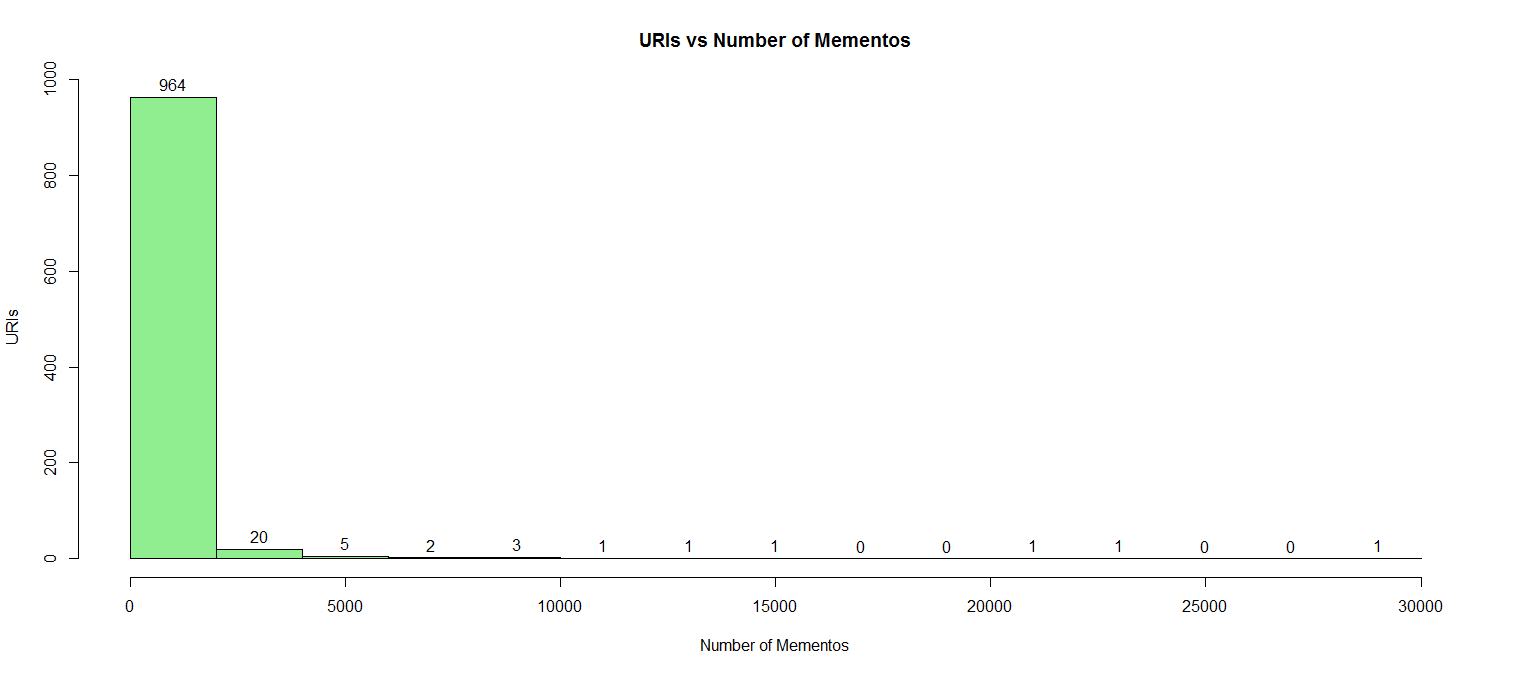
\includegraphics[width=0.90\textwidth]{mementoHistogram.png}
	\caption{URIs vs. Mementos}
	\label{fig:mementoHistogram}
\end{figure}


%%%%%%%%%%Chapter Exercises
\section{Question 3}
\subsection{Problem}Estimate the age of each of the 1000 URIs using the ``Carbon Date'' tool. For URIs that have at least one memento and an estimated creation date, create a graph with age (in days) on one axis and number of mementos on the other.
\subsection{Response}We used the provided Carbon Date\footnote{\url{http://ws-dl.blogspot.com/2013/04/2013-04-19-carbon-dating-web.html}} tool as the basis for our analysis.  SalahEldeen and Nelson \cite{salaheldeen2013carbon} describe the tool as ``a simple web application that estimates the creation date for a URI by polling a number
of sources of evidence and returning a machine-readable structure with their respective values''.  These information sources include bitly, topsy, Google, the ODU Memento aggregator and the HTTP response header. The tool, originally designed as a web service, was modified to accept file-based input (i.e., histogram.txt). Our Python program, \emph{EstimateAge}, described in Appendix \ref{chap:Python Source - EstimateAge}, performed line-by-line processing of the input file to identify the URLs with mementos. Once identified, the URL was passed to the main processes of Carbon Date to retrieve the estimated creation date.  Sample output is shown in Figure \ref{fig:CarbonDateSampleOutput}. If an estimated creation date was returned, the date was recorded in a text file (i.e., uri\_age.txt) along with the URI, number of mementos and calculated age in days. The format of the file is shown in Table \ref{tab:uriage}. We used the graphing functions in R to create a scatter plot as shown in Figure \ref{fig:scatterplot} which presents the relationship between the age of the URI and the number of mementos. The positive slope of the blue regression line indicates a strong relationship between the age of the URI and the number of expected mementos. Basically, older URIs would have accumulated more mementos over time.

\begin{figure}[htbp]
	\centering
		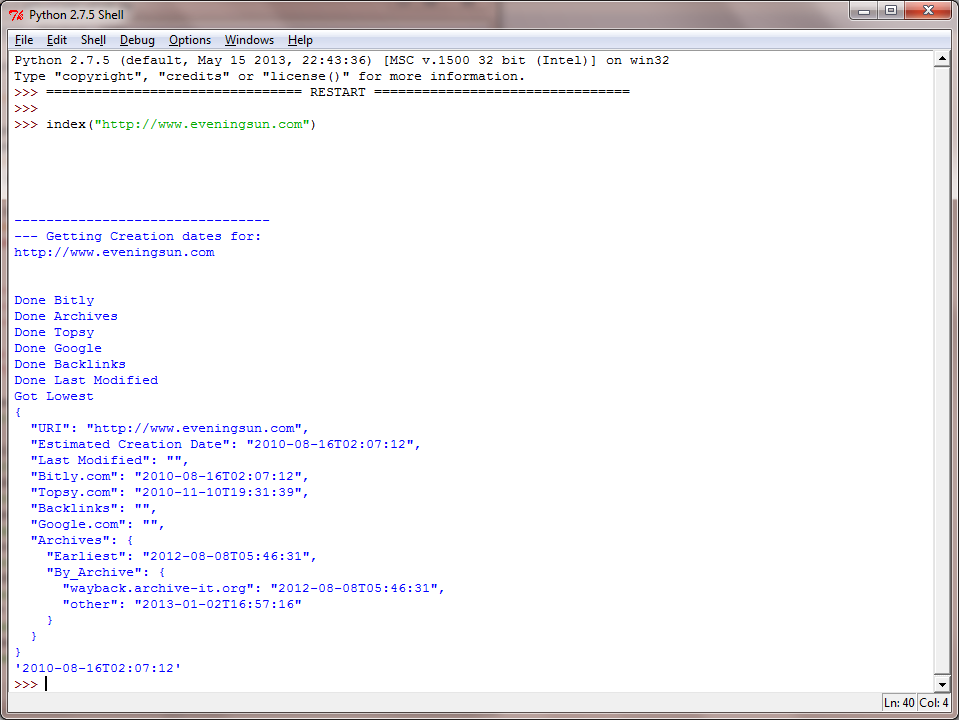
\includegraphics[width=0.90\textwidth]{CarbonDateSampleOutput.png}
	\caption{Carbon Date Sample Output}
	\label{fig:CarbonDateSampleOutput}
\end{figure}

\begin{table}[htbp]
\centering
    \begin{tabularx}{\textwidth}{X|r|l|r}
    \hline
    URI                                        & Mementos & Creation Date       & Age  \\ \hline
    \url{http://investmentwatchblog.com/}      & 287      & 2010-02-12T22:06:49 & 1316 \\ \hline
    \url{http://whithererehwon.wordpress.com/} & 2        & 2012-09-22T23:02:43 & 363  \\ \hline
    \url{http://maxcouti.blogspot.com/       } & 23       & 2008-05-18T15:07:07 & 1952 \\ \hline
    \end{tabularx}
    \caption{Format of uri\_age.txt}
		\label{tab:uriage}
\end{table}

\begin{figure}[htbp]
	\centering
		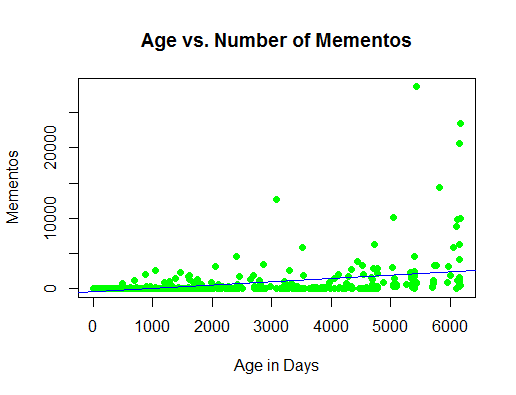
\includegraphics[width=0.90\textwidth]{scatterplot.png}
	\caption{Age vs. Number of Mementos}
	\label{fig:scatterplot}
\end{figure}

\end{savenotes}

% produce the bibliography for the citations in your paper.
\bibliographystyle{abbrv}
\bibliography{cmccoy}

\appendix
\addcontentsline{toc}{chapter}{Appendices}

%%Appendix A
\chapter{Python Source for extractLinks.py} \label{chap:Python Source - Extract Links}
\input{extractLinks.py}
\chapter{Python Source for getTimeMaps.py} \label{chap:Python Source - Get TimeMaps}
\input{getTimeMaps.py}
\chapter{R Source for Histogram} \label{chap:R Source - Histogram}
\input{histogram.r}
\chapter{Python Source for estimateAge.py} \label{chap:Python Source - EstimateAge}
\input{estimateAge.py}
\chapter{R Source for Scatterplot} \label{chap:R Source - Scatterplot}
\input{uri_age.r}



\end{document} 
%%%%%%%%%%Ed of report
